%----------------------------------------------------------------------------
%----------------------------------------------------------------------------
Suppose the solution, $\ket{\Psi}$, to (\ref{one dynamics}) is known at N+1 points from $t_0$ to $t_N$ where $t_i<t_j$ when $i<j$ $\forall$  $i,j \in \{0,1,\cdots,N\}$. Let $\ket{n}_i$ be the value of the nth component ($n \in \{ 0,1,2 \}$) of the solution, $\ket{\Psi}$, at time $t_i$. Consider the cost function
%----------------------------------------------------------------------------
\begin{equation}
\Phi
=
w\Phi_{residue}
+
\Phi_{intermediate}
\label{cost}
\end{equation}
%----------------------------------------------------------------------------
where
%----------------------------------------------------------------------------
\begin{equation}
\Phi_{residue}
=
P_0(t_N)
+
P_1(t_N).
\label{residue cost}
\end{equation}
%----------------------------------------------------------------------------
%----------------------------------------------------------------------------
\begin{equation}
\Phi_{intermediate}
=
\sum_i^N
P_1(t_i).
\label{int cost}
\end{equation}
%----------------------------------------------------------------------------
and $w$ is some weight factor.
%----------------------------------------------------------------------------
%----------------------------------------------------------------------------
A MathCAD program is used to minimize (\ref{cost}) as a function of $\sigma_\alpha$ (or $\sigma_\beta$), $A$, $B$, and $\Delta_\alpha$ for a system initially in the ground state over the time interval $[0,30]$ ($t_0 = 15$). A fourth-order Runge-Kutta fixed-step method is used to find the solution at 5000 points in the time interval. The MathCAD function ``Minimize'' is used to find the optimal solution.

After some initial runs, some symmetries in the solutions prompted the following reduction of variables: $\sigma_\alpha=\sigma_\beta=2$ and $A=B$; thus, the solution space is two dimensional, namely $\Delta_{\alpha}$ and $A$. Figure \ref{solution 2 pulses} shows the pulse sequence which minimized the cost function and figure \ref{solution 2 energy levels} show the resulting motion in $\braket{\Psi}{\Psi}$. In fact, a family of local optima exist. These optima improve, in general, as pulse amplitude increases. Figure \ref{solution 2-stronger energy levels} shows an example of an optimum where the pulses used have nearly twice the amplitude as the pulses shown in figure \ref{solution 2 pulses}.

The pulse sequence in Figure \ref{solution 2 pulses} is called the STIRAP pulse sequence in the literature \cite{Sola:1999a}. Its interesting properties include a ``counter--intuitive'' pulse sequence and the near zero population of the intermediate state during the entire process while the ground and upper state undergo inversion. One would expect the pulse taking the porbability up the ladder from the ground state to the first excited state should go first. In Figure \ref{solution 2 pulses} we see that the pulse sequence is reversed (hence the term ``counter--intuitive''); however, notice that there is significant overlap. 
%----------------------------------------------------------------------------
%----------------------------------------------------------------------------
% solution_2_pulses.tex
% by Troy Hix, March 2005
%----------------------------------------------------------------------------
\begin{figure}
\centering
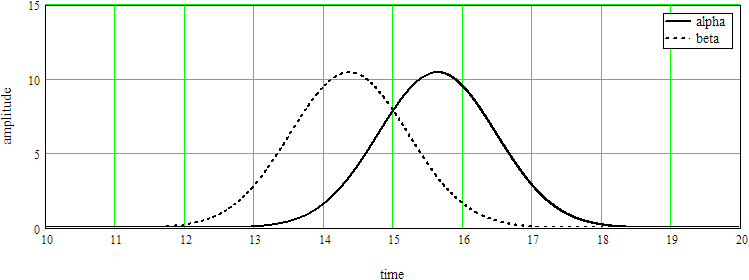
\includegraphics[width=5.00in]
{solution_2_pulses/solution_2_pulses.png}\\
\caption[Two color optimal pulse sequence (STIRAP)]{Two color optimal pulse sequence (STIRAP). With $\sigma_{\alpha}=\sigma_{\beta}\equiv 2$, the optimization program produced $\Delta_\alpha=-1.26997923288$ and $A=10.4616402919$ (14.179 times the area of the $\pi$--pulse) while $w$ was set to $10^8$. Note that although $\Delta_\alpha<0$, reflecting the fact that $\beta$ precedes $\alpha$, the pulses significantly overlap.}
\label{solution 2 pulses}
\end{figure} 
%----------------------------------------------------------------------------

%----------------------------------------------------------------------------
%----------------------------------------------------------------------------
% solution_2_pulses.tex
% by Troy Hix, March 2005
%----------------------------------------------------------------------------
\begin{figure}
\centering
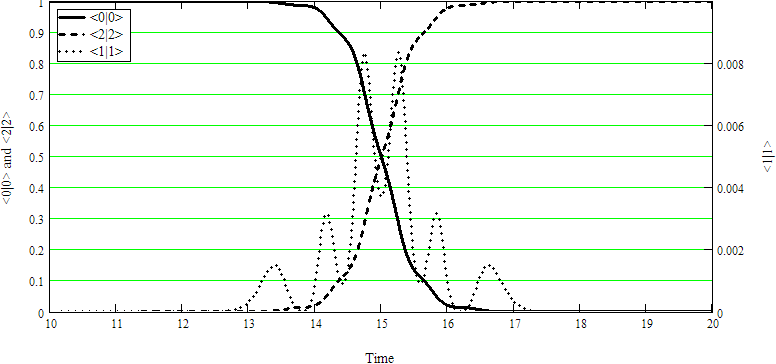
\includegraphics[width=5.00in]
{solution_2_energy_levels/solution_2_energy_levels.png}\\
\caption[Two color optimal solution]{Two color optimal solution. $\braket{\Psi}{\Psi}$'s behavior at the optimum using the pulse sequence from Figure \ref{solution 2 pulses}. Note that $\braket{0}{0}$ and $\braket{2}{2}$ are shown at a different scale than $\braket{1}{1}$. This solution effectively transfers population directly from the ground state to the second excited state without significantly populating the first excited state.}
\label{solution 2 energy levels}
\end{figure} 
%----------------------------------------------------------------------------

%----------------------------------------------------------------------------
%----------------------------------------------------------------------------
%----------------------------------------------------------------------------
% solution_2_pulses.tex
% by Troy Hix, March 2005
%----------------------------------------------------------------------------
\begin{figure}
\centering
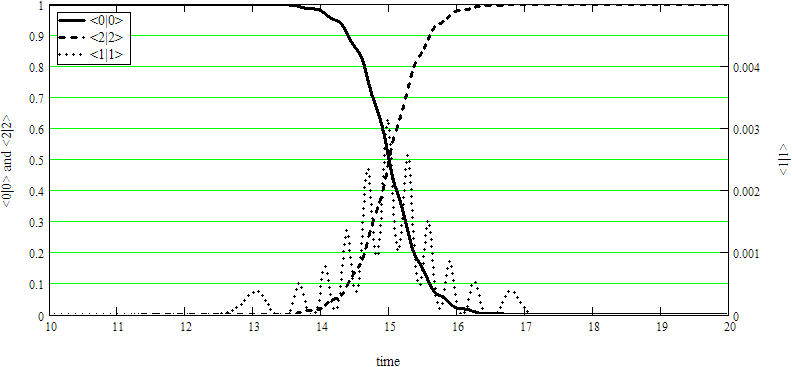
\includegraphics[width=5.00in]
{solution_2-stronger_energy_levels/solution_2-stronger_energy_levels.png}\\
\caption[Two color optimal solution - increased pulse amplitude]{Two color optimal solution - increased pulse amplitude. $\braket{\Psi}{\Psi}$'s behavior at an optimum with increased pulse amplitudes. Note that $\braket{0}{0}$ and $\braket{2}{2}$ are shown at a different scale than $\braket{1}{1}$. Notice the decrease in the average height of $\braket{1}{1}$ when compared to $\braket{1}{1}$ in figure \ref{solution 2 energy levels}. For this solution $\Delta_{\alpha}=-1.3146820926$ and $A=19.5606505329$ (26.511 times the area of the $\pi$--pulse).}
\label{solution 2-stronger energy levels}
\end{figure} 
%----------------------------------------------------------------------------

%----------------------------------------------------------------------------
